\begin{slide}{Use Cases}
\begin{columns}
  \begin{column}{0.6\textwidth}
    \begin{itemize}
      \item<2-> Smart email replies in Google \emph{Inbox}
      \item<3-> Emails mapped to ``thought vectors''
      \item<4-> LSTMs synthesize valid replies
    \end{itemize}
  \end{column}
  \begin{column}{0.4\textwidth}
    \begin{figure}
      \onslide<2->{
        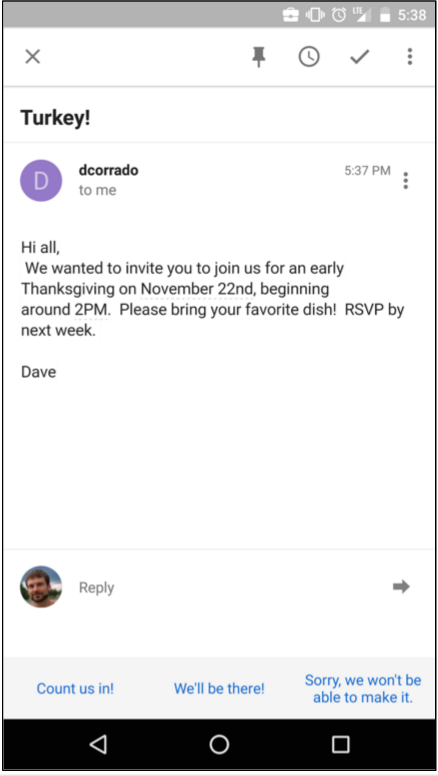
\includegraphics[scale=0.25]{emails}
      }
    \end{figure}
  \end{column}
\end{columns}
{\tiny Source: http://googleresearch.blogspot.de/2015/11/computer-respond-to-this-email.html}
\end{slide}

\begin{frame}
  \frametitle{Use Cases}
  \begin{itemize}
  \item<2-> Google DeepMind now using TensorFlow
  \item<3-> Already for \emph{AlphaGo}
  \item<4-> According to a DeepMind SWE reasons are:

    \begin{itemize}
      \item<5-> Python,
      \item<6-> Integration with Google Cloud Platform,
      \item<7-> Support for TPUs,
      \item<8-> Ability to run on many GPUs.
    \end{itemize}
  \end{itemize}
  \onslide<3->{
  \begin{center}
    
\includegraphics[scale=0.15]{alphago}\\
    \vspace{0.1cm}
    \tiny Source:
      https://deepmind.com/css/images/opengraph/alphago-logo.png
  \end{center}
  }
\end{frame}

%%% Local Variables:
%%% mode: latex
%%% TeX-master: "../presentation"
%%% End:
